


\documentclass[main]{subfiles}

\begin{document}


\chapter{Results \& Insights}


This chapter includes saliency metric and qualitative results from testing the method panel on ImageNet data and pre-trained CNN models. Insights are compared with existing insights in the literature and summarised at the end of the chapter.

\section{Experiment Notes}

\subsection{Sample Sizes}  \label{sec:data_collection}
A set of 300 attributions for the full method panel took around 10 hours to collect and evaluate using a Nvidia GTX-1080 GPU. LIME was thought to be a key bottleneck due to its perturbation-based approach, but analysis in Section \ref{sec:perform} showed GradCAM was also slow in attribution. After several hundred attributions the process became very slow and would have to be restarted from that point (possibly due to a GPU memory leak in method internals). These performance considerations meant only 1000 instances out of 50,000 available in the validation set were ever used for evaluation. This was at least the same 1000 instances for all methods, and different dimensions were added to generate insights regardless: different attribution thresholds, and subsetting the results for high confidence (p $>0.9$) vs low confidence model predictions.

\subsection{Software Availability}

Code for the testing framework is available on GitHub and is intended to be made public after improving model agnosticity and cleaning up dependencies and file structures. The framework has modular support for attribution methods (provided they are compatible with image data and return an input-space representation of their explanation) and modular support for other saliency metrics.


\subsection{Testing on Multiple Architectures} \label{sec:shap_note}

Some limitations were encountered on SHAP for ResNet50 and InceptionV3 architectures. Other methods were successfully tested on other models with results below, though the bug in SHAP was not ultimately resolved. The impact of this obstacle is discussed in Section \ref{sec:compatibility}.

\section{Saliency Metric Results}
\subsection{VGG16} \label{sec:vggExp}

Figure \ref{vggAfig} shows IOU and IOU* statistics for a 1000-instance sample explaining VGG16 model predictions. The 1000 instances are broken up into high confidence (top row) and low confidence predictions (bottom row). Error bars indicate one standard deviation from the mean result displayed by bar height, and are later used as a proxy of method consistency (Section \ref{sec:consistency}). For this experiment setup, a threshold of 0.5 standard deviations was applied to the attribution output for IOU and 1 standard deviation for IOU*.\\

\vspace{0.1in}
\noindent Some initial observations from Figure \ref{vggAfig} (others discussed in \ref{sec:saliency_insights}):
\begin{itemize}
\item Results are similar for high vs low confidence predictions, with LIME's variance being one noticeable difference.
\item SHAP and DeepLift perform similarly on IOU but not IOU*.
\item GradCAM scores lower on these metrics though is visually less noisy than DeepLIFT and SHAP.
\end{itemize}


\newpage

%\vspace{2in}

\begin{figure}[h]\centering
\vfill
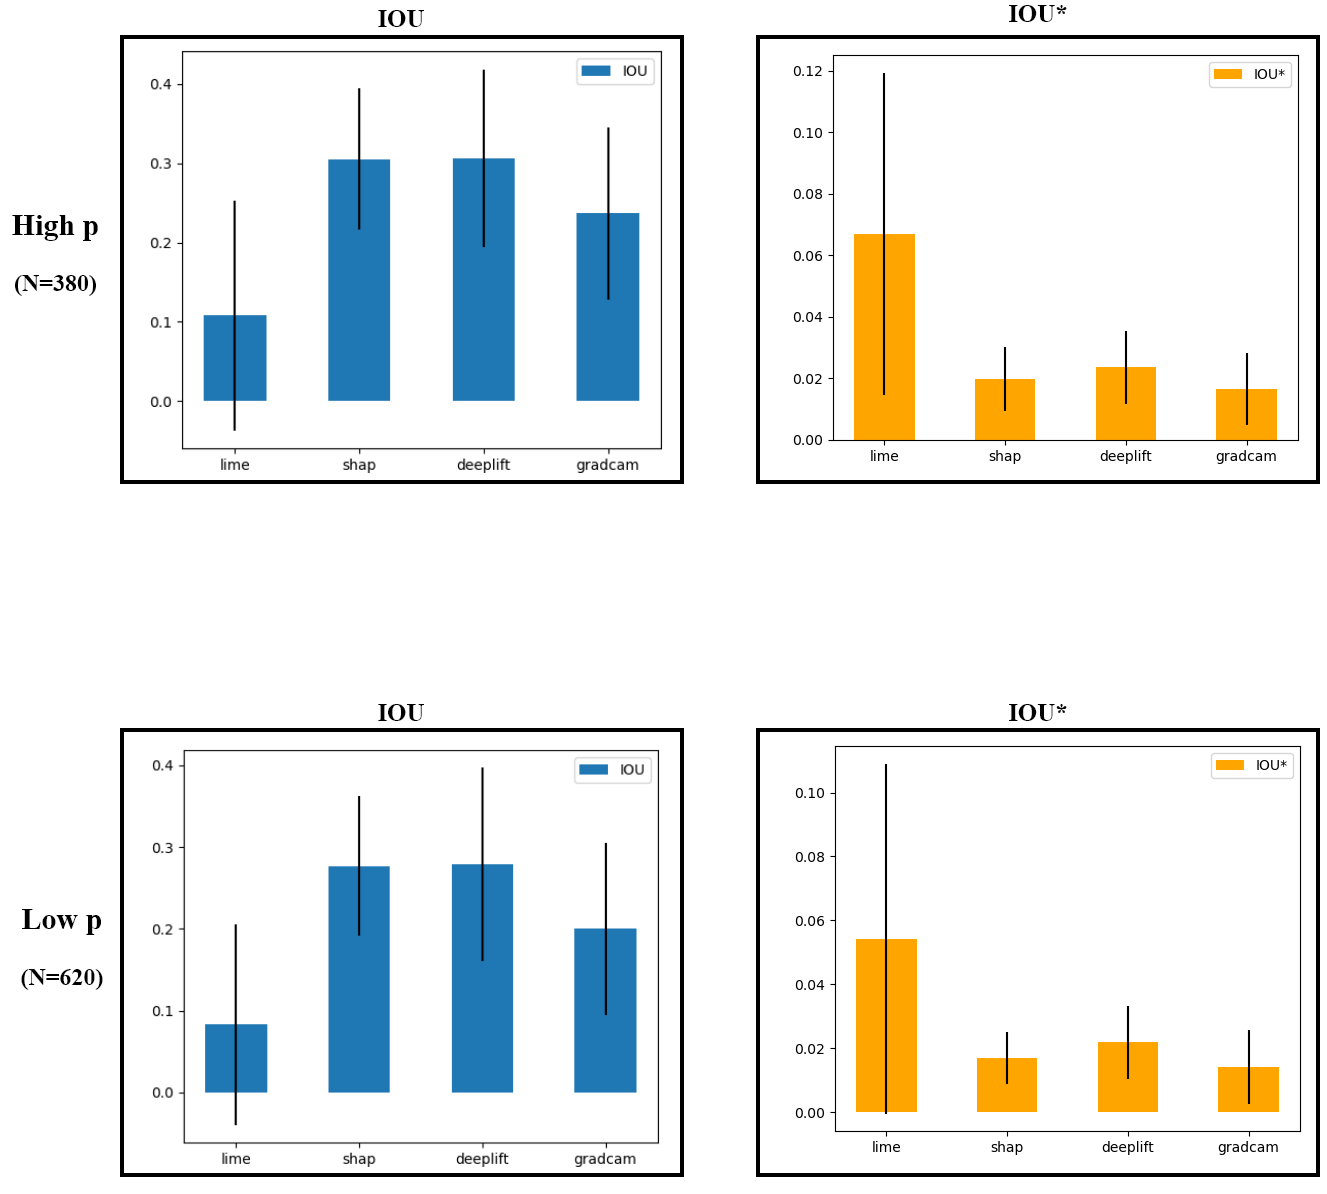
\includegraphics[scale=0.32]{vgg_0_5_and_1.png}
\caption{Results for a 1000-instance attribution sample of VGG16. }
\label{vggAfig}
\vfill
\end{figure}

In Appendix C, Figure \ref{vggExtraFig} shows comparatively identical results for a smaller sample (N=300) with a different threshold set: 1 for IOU and 2 for IOU*.

\newpage


\subsection{InceptionV3}

\begin{figure}[h]
\centering
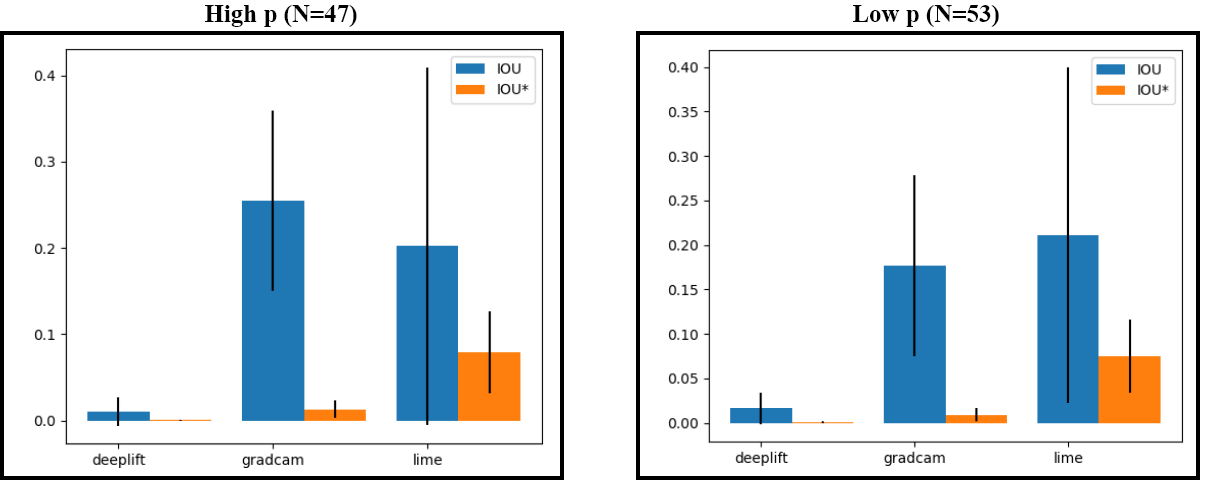
\includegraphics[scale=0.35]{inception.png}
\caption{Results for a 100-instance attribution sample of InceptionV3. }
\label{inceptionFig}
\end{figure}

Model results on this page are only considered auxiliary, since SHAP was excluded from the panel (\ref{sec:shap_note}). The lower sample size was a compromise on allocated experiment time due to the longer attribution time for these models.

The most interesting observation here is that GradCAM under-performs on low confidence predictions compared to LIME. Given the high variance and low sample size these results are tentative however. DeepLIFT's non-performance is also analysed in the next section.

\subsection{ResNet50}

\begin{figure}[h]
\centering
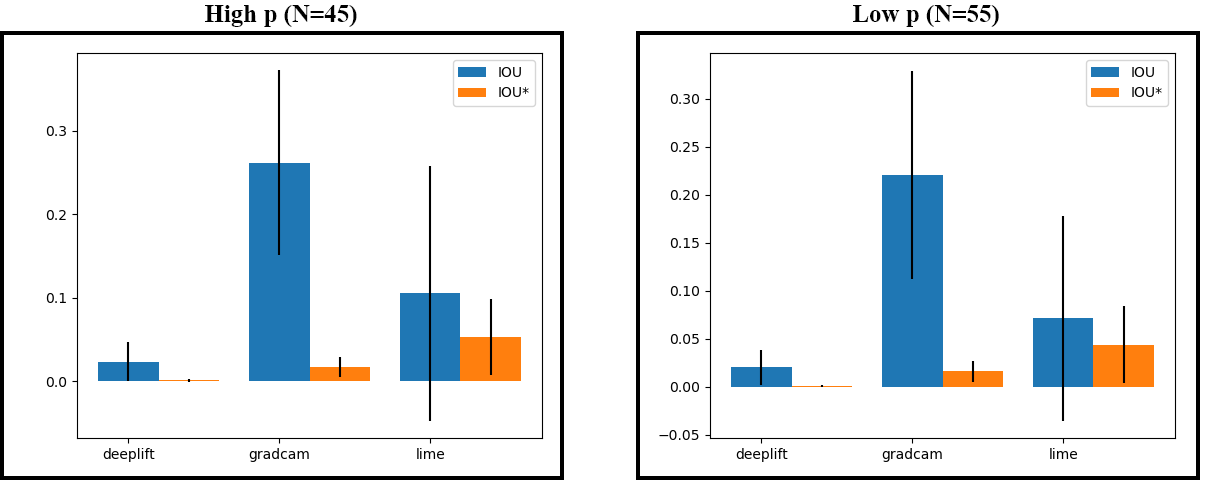
\includegraphics[scale=0.35]{resnet.png}
\caption{Results for a 100-instance attribution sample of ResNet50. }
\label{resnetFig}
\end{figure}

These results are more like the VGG16 results in Figure \ref{vggAfig}. Here, no noticeable difference between high and low confidence subsamples is observed, and GradCAM out-performs LIME on IOU but not IOU*, as in the VGG16 results.


\newpage
\subsection{Insights from Saliency Metrics} \label{sec:saliency_insights}

\subsubsection{What did pixel-wise attribution (IOU) highlight?}
SHAP and DeepLIFT were the best performers on VGG16 with variance in LIME noticeably high and GradCAM performing not quite as well in terms of mean IOU. However, both SHAP and DeepLIFT failed on other models, which is a problem explored further in Section \ref{sec:compatibility}.

The DeepLIFT saliency results contradict empirical results on its visual saliency. Its attributions were visually much noisier than others and this may have inflated its IOU comparatively if enough of the noise was in the ground truth region. 

On balance, when considering across-model result generalisation (where GradCAM excels) and visual saliency (where SHAP and GradCAM excel), both SHAP and GradCAM should be considered superior for saliency in terms of pixel-level detail or `discriminatory power'.
 
The impact of thresholding also appeared to make no difference to the ordinal differences between methods (Appendix C). It seems that a higher threshold led to only smaller IOU magnitude rather than a change in one method's performance relative to another. 

%The theory of noise in DeepLIFT is not supported by the higher threshold results in Appendix C, since intuitively its performance would drop with the bias removed.

\subsubsection{What did strength of attribution (IOU*) highlight?}

The IOU* metric results unfortunately did not derive much further insight. However, a couple of observations were still made:
\begin{itemize}
\item LIME outperformed all other methods on IOU*, but since superpixel regions are broadly brushed with the same attribution score, this can be attributed to some bias introduced from the methodology.
\item DeepLIFT out-performed SHAP and GradCAM on the VGG16 results though this is possibly due to higher noise across the input space.
\end{itemize}

\noindent How strongly individual pixels are weighted may need to be rewarded more generously: attributions are only bounded between 0 and 1 (with absolute value taken), and so small regions of intensity are probably averaged out by the denominator union array. A suggestion for future work on weighted saliency metrics is to use larger weighting and/or an alternative to IOU.

\newpage
\section{Other Criteria}
\subsection{Performance} \label{sec:perform}


\begin{figure}[h]\centering
\vfill
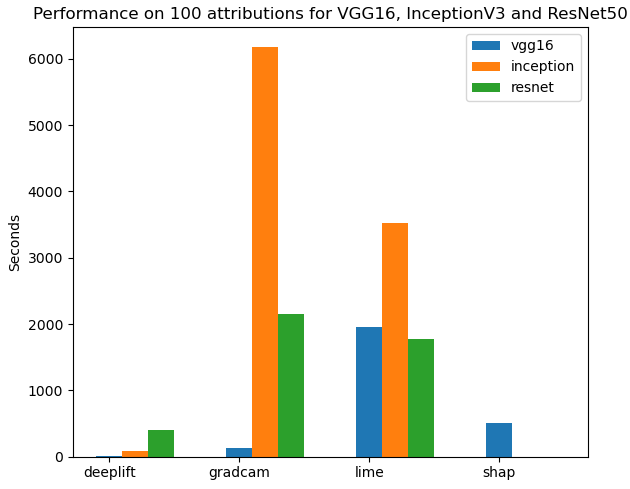
\includegraphics[scale=0.6]{performance.png}
\caption{Performance/speed in seconds for VGG16, InceptionV3, and ResNet50. }
\label{performFig}
\vfill
\end{figure}

\noindent Some insights from performance measurements in Figure \ref{performFig} are described here.

These results are correlated with the time the underlying model takes to calculate a prediction, which is itself a function of the number of model layers and parameters. This is controlled across the panel at least, so the relative performance of each method can still be highlighted (and to some extent performance correlation with model complexity). For example, DeepLIFT's claims of fast performance due to requiring only a single backwards pass are supported by these results. It was also extremely fast for InceptionV3 and much slower on ResNet50, which cannot be explained easily, though two possible reasons are the denser convolutional layers in ResNet50 or a method internal bug.

A surprising insight is that GradCAM performed much worse than LIME for a 100-instance sample. A standard assumption in the literature is that perturbation techniques are necessarily much slower than other approaches. Further analysis however with Guided Backpropagation removed from the Guided GradCAM method used here saw its performance on InceptionV3 reduce from over 6000 seconds (Figure \ref{performFig}) to roughly 200 for the same sample size. This shows that the discriminative version of GradCAM comes at a significant performance cost for architectures with many layers, and similar or worse results would have been seen for SHAP for this project's methodology to apply Guided Backpropagation to its outputs as well.


\newpage
\subsection{Consistency}\label{sec:consistency}
Analysis is provided below on consistency across attributions. Table \ref{consistencytable} lists standard deviations for the method panel from the 1000-instance experiment run on VGG16 (error bars in Figure \ref{vggAfig}):

\begin{table}[htbp]
\centering
\begin{tabular}{l|l|l|l|l|}
\cline{2-5}
                  & \multicolumn{2}{c|}{\textbf{IOU}} & \multicolumn{2}{c|}{\textbf{IOU*}} \\ \cline{2-5} 
                  & \textbf{High p}           & \textbf{Low p}          & \textbf{High p}           & \textbf{Low p}           \\ \hline
\multicolumn{1}{|l|}{LIME}     & 0.145            & 0.122          & 0.052            & 0.055           \\ \hline
\multicolumn{1}{|l|}{SHAP}      & 0.089            & 0.085          & 0.010            & 0.008           \\ \hline
\multicolumn{1}{|l|}{DeepLIFT}  & 0.112            & 0.118          & 0.012            & 0.011           \\ \hline
\multicolumn{1}{|l|}{GradCAM}   & 0.109            & 0.105          & 0.012            & 0.012           \\ \hline
\end{tabular}

\caption{Standard deviations on 1000-instance saliency metrics.}
\label{consistencytable}

\end{table}

\noindent LIME suffers the highest variance over the sample, which corroborates findings by Alvarez-Melis \& Jaakkola (2018) (Section \ref{sec:existing_criteria}) that LIME and model-agnostic, perturbation-based techniques generally are more prone to instability than gradient-based techniques. 

For other methods, results were consistent across high and low confidence predictions, which was an unexpected finding. This may have been because of a certain baseline level of  noise that each method outputs, meaning underlying model confusion did not translate into lower IOU or IOU* on average.

For consistency across models, it was noted in Section \ref{sec:saliency_insights} that DeepLIFT performed strongly on VGG16 and very poorly on more complex architectures. This was therefore a strength of LIME and GradCAM: they performed slightly worse on IOU in the VGG16 experiment but better on more complicated architectures. In terms of consistency though, LIME's attributions increased in variance on the saliency metrics for the more complicated architectures (Figures \ref{inceptionFig} and \ref{resnetFig}). This is another blight on its reputation for instability.


\newpage
\subsection{Ease of Adaption} \label{sec:compatibility}
Observations on each method's implementation considerations are made in this section. Reference is made to their hyperparameter complexity and model compatibility, which together can be summarised as ease of adaption. In the following chapter, a higher level comparison of each method's approach (and related implementation considerations) is also provided.

\subsubsection{GradCAM}
A note on GradCAM made was that its performance significantly deteriorates when replacing its localisation `heatmap' formulation with the discriminative upgrade proposed by the authors (i.e. multiplied with Guided Backpropagation). This is a compromise that practitioners can be aware of: for individual explanations, it may be desirable to use Guided GradCAM to see a higher resolution explanation, since at-scale evaluation is not a concern. For explaining many model predictions, or where localisation is more important to the use case than individual patterns or edges, the variant without Guided Backpropagation should be preferred.

\noindent Other insights about GradCAM's use cases:
\begin{itemize}
\item GradCAM's explanations were consistently visually salient, and also consistent in the saliency metric results. This could be because it is inherently designed for CNN architectures: the target of the final convolutional layer where the features are intuitively represented in the most abstract form seems to lead to more visually appealing explanations for model behaviour.
\item GradCAM is suited as an `off the shelf' option for CNN architectures. It requires no modification to internal gradient or backpropagation operations: a strength over backpropagation methods like DeepLIFT.
\end{itemize}


\subsubsection{DeepLIFT}

DeepLIFT performed strongly on VGG16 but appeared to fail completely on more complex architectures. The reason may be due to the implementation: DeepLIFT requires an architectural modification that has to be done for each layer type, which is to implement the custom backpropagation function that incorporates reference activations (i.e. transform gradients into attributions that represent differences from those reference activations). For this project, the implementation relied upon may not have been able to handle ResNet's residual layers or Inception's layer modules. Full neural network compatibility may be a theoretically true claim by the authors but these caveats (and determining reference activations) are a major practical drawback.

%DeepLIFT's speed on architectures with fewer convolutional layers was not noticeably worse, which possibly indicates it is suited for `network in network' architectures like InceptionV3. For solely convolutional architectures, it is arguably not the best in the panel (based on visual saliency and the saliency metrics). SHAP 

%"Methods like LRP and DeepLift replace gradients with discrete gradients and still use a modified form of backpropagation to compose discrete gradients into attributions" IG

\subsubsection{SHAP}
The difficulty also observed in applying SHAP to more complicated model architectures suggests that other practitioners may have similar difficulties with their own models. SHAP is a higher level \textit{specification} of an explanation method rather than a particular formulation (Section \ref{sec:othermodelag}) which makes it difficult to evaluate independently of its model-specific approximations.

One of those model-specific approximations is based on Integrated Gradients and was the one relied upon in this project. This SHAP implementation saw almost identical results to DeepLIFT, in terms of saliency in Figure \ref{vggAfig}, and consistency in Table \ref{consistencytable}). This supports the suggestion that DeepLIFT is a more practical approximation of Integrated Gradients with a similar level of accuracy (Ancona et al. (2017), Section \ref{sec:existing_studies}).

SHAP's key implementation requirements are a background sample of predictions needed to estimate the expectation of model output, and the choice of a layer target to explain. Neither of these were difficult to specify, though the choice of layer is somewhat arbitrary compared to GradCAM's specification of the final convolutional layer.

Though it couldn't be practically evaluated on other architectures, its visual saliency on VGG16 was appealing, and it is notable that SHAP highlighted different features to other methods for the same prediction (e.g. Figure \ref{panel2img}). SHAP's software package also provides approximations for a number of model families \cite{shaprepo}, which was part of the motivation for its initial description as a model-agnostic method.


\subsubsection{LIME}
Although it is fully model-agnostic and therefore had fewer implementation difficulties, LIME has two important hyperparameters that have not been mentioned so far in discussion. This is the number of training samples of locally perturbed input features taken, as well as the number of features (superpixels) for each sample. Both were taken near the authors' defaults, as a suggested compromise between performance and accuracy \cite{limerepo}.

The superpixel-based output of LIME is better suited for \textit{localisation} saliency measures (not targeted by this project). In a sense LIME was slightly misrepresented by how it was adapted for pixel-wise attribution, with superpixel weights brushed over all pixels in each bounded region. However, this adaption step was necessary for evaluation with other methods, and superpixel weights still represent input space attributions.
%"While we have made a case for model agnosticism, this approach is not without its challenges. For example, getting a global understanding of the model may be hard if the model is very complex, due to the trade-off between flexibility and interpretability. To make matters worse, local explanations may be inconsistent with one another, since a flexible model may use a certain feature in different ways depending on the other features. In Ribeiro et al. (2016) we explained text models by selecting a small number of representative and non-redundant individual prediction explanations obtained via submodular optimization, similar in spirit to showing prototypes (Kim et al., 2014). However, it is unclear on how to extend this approach to domains such as images or tabular data, where the data itself is not sparse. In some domains, exact explanations may be required (e.g. for legal or ethical reasons), and using a black-box may be unacceptable (or even illegal). Interpretable models may also be more desirable when interpretability is much more important than accuracy, or when interpretable models trained on a small number of carefully engineered features are as accurate as black-box models."  Model-Agnostic Interpretability of Machine Learning

% mention low performance on oterh model archtiectures from Lit Review (ancona)

\newpage
\section{Summary of Insights}
\subsection{Quantitative}

\begin{table}[h]
\begin{tabular}{l|l|l|l|}
\cline{2-4}
                                        & \multicolumn{1}{c|}{\textbf{\begin{tabular}[c]{@{}c@{}}Saliency (IOU, IOU*)\\    (Section \ref{sec:saliency_insights})\end{tabular}}} & \multicolumn{1}{c|}{\textbf{\begin{tabular}[c]{@{}c@{}}Consistency\\ (Section \ref{sec:consistency})\end{tabular}}} & \multicolumn{1}{c|}{\textbf{\begin{tabular}[c]{@{}c@{}}Performance\\ (Section \ref{sec:perform})\end{tabular}}} \\ \hline
\multicolumn{1}{|l|}{\textbf{LIME}}     & \begin{tabular}[c]{@{}l@{}}Low IOU; High IOU* \\ explained by superpixel \\ weighting\end{tabular}                    & \begin{tabular}[c]{@{}l@{}}Poor over the \\ sample; Unstable\end{tabular}                           & \begin{tabular}[c]{@{}l@{}}Very slow for all \\ three models\end{tabular}                       \\ \hline
\multicolumn{1}{|l|}{\textbf{SHAP}}     & \begin{tabular}[c]{@{}l@{}}High IOU; failed on \\ other models; \\ visually salient\end{tabular}                       & \begin{tabular}[c]{@{}l@{}}Consistent for \\ model confidence\end{tabular}                          & \begin{tabular}[c]{@{}l@{}}Moderate speed; \\ incomplete results\end{tabular}                   \\ \hline
\multicolumn{1}{|l|}{\textbf{DeepLIFT}} & \begin{tabular}[c]{@{}l@{}}High IOU and IOU*;\\ failed on other models; \\ noisy explanations\end{tabular}                          & \begin{tabular}[c]{@{}l@{}}Consistent for \\ model confidence\end{tabular}                          & \begin{tabular}[c]{@{}l@{}}Fast; results also \\ incomplete\end{tabular}                        \\ \hline
\multicolumn{1}{|l|}{\textbf{GradCAM}}  & \begin{tabular}[c]{@{}l@{}}Average IOU and \\ IOU*; visually salient\end{tabular}                                      & \begin{tabular}[c]{@{}l@{}}Consistent for \\ model confidence \\ and across models\end{tabular}     & \begin{tabular}[c]{@{}l@{}}Guided-GradCAM\\  = very slow; \\ Grad-CAM = fast\end{tabular}       \\ \hline
\end{tabular}
\caption{Summary of quantitative evaluation insights.}
\end{table}

\subsection{Qualitative}

\begin{table}[htbp]
\begin{tabular}{l|l|l|}
\cline{2-3}
                                        & \multicolumn{1}{c|}{\textbf{Relative Strengths}}                                                                                          & \multicolumn{1}{c|}{\textbf{Relative Weaknesses}}                                                                           \\ \hline
\multicolumn{1}{|l|}{\textbf{LIME}}     & \begin{tabular}[c]{@{}l@{}}Full model compatibility;\\ ease of adaption\end{tabular}                                                      & \begin{tabular}[c]{@{}l@{}}Explanation instability;\\ accuracy-linked hyperparameters\end{tabular}                                  \\ \hline
\multicolumn{1}{|l|}{\textbf{SHAP}}     & \begin{tabular}[c]{@{}l@{}}Model and task compatibility;\\ theoretic basis\end{tabular}                                                   & \begin{tabular}[c]{@{}l@{}}Uncertain hyperparameter choice;\\ competing approximations (+ bugs)\end{tabular}                \\ \hline
\multicolumn{1}{|l|}{\textbf{DeepLIFT}} & \begin{tabular}[c]{@{}l@{}}Neural network compatibility;\\ task compatibility\end{tabular}                                                & \begin{tabular}[c]{@{}l@{}}Implementation complexity\\ (increasing in model complexity)\end{tabular}                        \\ \hline
\multicolumn{1}{|l|}{\textbf{GradCAM}}  & \begin{tabular}[c]{@{}l@{}}Low hyperparameter complexity;\\ flexibility in heatmap localisation \\ vs pattern discrimination\end{tabular} & \begin{tabular}[c]{@{}l@{}}Model inflexibility: designed for CNNs;\\ task inflexibility: suited for image data\end{tabular} \\ \hline
\end{tabular}
\caption{Summary of qualitative insights.}
\end{table}


\end{document}